\chapter{Комплекс функцийн дифференциалчлал}
\section{Уламжлал ба дифференциал. \\ \index{Уламжлал}
Эйлер-Даламберийн нөхцөл, \index{Эйлер-Даламберийн нөхцөл}
Голоморф функц}
Комплекс хувьсагчийн функцийн уламжлалын тодорхойлолт бодит хувьсагчийн функцийнх шиг формаль байдлаар өгөгдөнө.\index{Формаль уламжлал} $z_0$-цэгийн ямар нэг $U=U(z_0,\delta)=\{|z-z_0|<\delta\}$ орчинд нэг утгат $w=f(z)=u+iv$ функц тодорхойлогдсон байг. Удирдан хувьсах $z$ хэмжигдэхүүн өөрийн $U$ орчноос үл гарах бүх боломжит
$$\Delta z=z-z_0=(x-x_0)+i(y-y_0)=\Delta z+i\Delta y\neq 0$$
өөрчлөлт авч байг. $\Delta z$ өөрчлөлт бүрд харгалзах функцийн өөрчлөлт
$$\Delta w=\Delta f(z_0)=f(z)-f(z_0) =\Delta u+i\Delta v$$
байна гэж үзье. Функцийн $\Delta w$ өөрчлөлтийг удирдан хувьсах хэмжигдэхүүний $\Delta z$ өөрчлөлтөд хувааж $\Delta z\rightarrow 0$ байхаар хязгаарт шилжье. Хэрэв энэ хязгаар оршин байвал түүнийг\\ $w=f(z)$ функцийн $z_0$ цэг дээрх уламжлал гэж нэрлэх бөгөөд 
\begin{eqnarray} \label{3.1}
 \dfrac{dw}{dz}\Big |_{z=z_0}=f'(z_0)=\lim\limits_{\Delta z\rightarrow 0}\dfrac{\Delta w}{\Delta z}
\end{eqnarray}

тэмдэглэл хэрэглэнэ. 

$w=f(z)$ функц $z_0$ цэгийн ямар нэг $U=U(z_0,\delta)$ орчинд тодорхойлогдохын хамт түүний $\Delta w$ өөрчлөлтийг $\Delta z$-ийн хувьд шугаман $A\cdot \Delta z$ хэсэг ба $\Delta z$-тэй жишихэд дээд эрэмбийн төгсгөлгүй багасах хэмжигдэхүүний нийлбэрийн
\begin{eqnarray} \label{3.2}
 \Delta w=\Delta f(z_0)=A\cdot \Delta z+\circ (\Delta z)=A\cdot \Delta z+\alpha (\Delta z)\cdot \Delta z
\end{eqnarray}

дүрстэй бичигдэж байвал $w=f(z)$-ийг $z_0$ цэг дээр дифференциалчлагдах функц гэнэ. Энд $A$ тоо $\Delta z$-ээс үл хамаарах бөгөөд харин $\alpha (\Delta z)$ нь $\Delta z\rightarrow 0$ үед төгсгөлгүй бага функц, өөрөөр хэлбэл $\lim\limits_{\Delta z\rightarrow 0}\alpha (\Delta z)=0$, иймд $\circ (\Delta z)=\alpha (\Delta z)\cdot \Delta z$ нь $\Delta z$-тэй жишихэд дээд эрэмбийн төгсгөлгүй багасах хэмжигдэхүүн.
\begin{thm}
$w=f(z)$ функц $z_0$ цэг дээр дифференциалчлагдах зайлшгүй бөгөөд хүрэлцээтэй нөхцөл\index{Дифференциалчлагдах нөхцөл} нь уул функц $z_0$ дээр уламжлалтай, тухайлбал $A=f'(z_0)$ байх явдал мөн.
\end{thm}
\begin{prf}
\textbf{Зайлшгүй:} (\ref{3.2}) биелэгдэж байна гэдгээс
$$\frac{\Delta w}{\Delta z}=A+\frac{\circ (\Delta z)}{\Delta z}$$ бөгөөд $\Delta z \rightarrow 0$ үед 
$$A=\lim\limits_{\Delta z \rightarrow 0} \frac{\Delta w}{\Delta z}=w'(z_0)$$ болов. \\
\textbf{Хүрэлцээтэй нь:} $w'(z_0)$ оршин байна гэдгээс $\Delta z\rightarrow 0$ үед
$$\Delta w=A\cdot \Delta z+\alpha (\Delta z)\cdot \Delta z$$ болж батлагдлаа.
\hfill $\blacksquare$\end{prf}
$w=f(z)$ функцийн $z_0$ цэг дээрх дифференциал \index{Дифференциал} гэж
\begin{eqnarray}
 dw=df(z_0)=f'(z_0)dz
\end{eqnarray}-ийг нэрлэнэ. Дифференциал нь функцийн өөрчлөлтийн гол хэсэг.

Комплекс хувьсагчийн функцийн дифференциалчлагдах нөхцөл бодит хувьсагчийн функцийн дифференциалчлагдах нөхцөлөөс гадна нэмэлт нөхцөл шаардахыг дараах теорем харуулна.
\begin{thm}
Комплекс $w=f(z)=u(x,y)+iv (z,y)$ функц $z_0=x_0+iy_0$ цэгийн орчинд тодорхойлогдсон байг. Энэ функц $z_0$ цэг дээр дифференциалчдаглах зайлшгүй бөгөөд хүрэлцээтэй нөхцөл нь
\begin{enumerate}
    \item $u(x,y)$, $v(x,y)$ функцүүд $(x_0,y_0)$ цэг дээр дифференциалчлагдах,
    \item Эйлер-Даламберийн 
    \begin{equation}
\tag{E-D}
\dfrac{\partial u}{\partial x}=\dfrac{\partial v}{\partial y}, \qquad \dfrac{\partial u}{\partial y}=-\dfrac{\partial v}{\partial x}
\end{equation} нөхцөл $(x_0,y_0)$ цэг дээр биелэгдэх явдал мөн.
\end{enumerate}
\end{thm}
\begin{prf}
\textbf{Зайлшгүй:} (\ref{3.1}) биелэгдэж байг. 
$$\Delta f(z_0)=\Delta u+i\Delta v=f'(z_0)\Delta z+\circ (\Delta z)$$ бөгөөд $f'(z_0)=a+ib$, $\circ (\Delta z)= \alpha +i\beta$ гэж орлуулахдаа $a,b\in\mathbb{R}$, $\alpha$, $\beta$ нь $\Delta z\rightarrow 0$ үед дээд эрэмбийн төгсгөлгүй багасах бодит тоонууд гэж тооцъё.

Тэгтэл 
\begin{eqnarray}
 \Delta u+i \Delta v=(a+ib) (\Delta x+i\Delta y)+\alpha +i\beta
\end{eqnarray} болж 
\begin{eqnarray}
 \Delta u=a \Delta x-b\Delta y+\alpha, \qquad \Delta v=b\Delta x+a\Delta y +\beta
\end{eqnarray}

эндээс $u(x,y)$, $v(x,y)$ нь $(x_0,y_0)$ цэг дээр дифференциалчлагдах функцүүд болох нь батлагдаж түүнчлэн (3.5)-аас
$$a=\dfrac{\partial u}{\partial x}=\dfrac{\partial v}{\partial y}, \quad b=\dfrac{\partial u}{\partial y}=-\dfrac{\partial v}{\partial x}$$
гээд (E-D) гарч ирлээ. Ингэж теоремын зайлшгүй нөхцөл батлагдав. Теоремын нөхцөлүүдийн хүрэлцээтэйг баталъя.
1) ба 2) нөхцөл биелэгдсэн байг, өөрөөр хэлбэл
$$
\begin{cases}
\Delta  u=\dfrac{\partial u}{\partial x}\Delta x+\dfrac{\Delta u}{\Delta y}\Delta y+\alpha_1\Delta x+\alpha_2\Delta y\\
\Delta v=\dfrac{\partial v}{\partial x}\Delta x+\dfrac{\Delta v}{\Delta y}\Delta y+\beta_1\Delta x+\beta_2\Delta y
\end{cases}
$$ 
Энд $\alpha_1$, $\alpha_2$, $\beta_1$, $\beta_2$ нь $\Delta x$, $\Delta y$-ийн тэг рүү тэмүүлэх нөхцөлд тэг рүү тэмүүлэх хэмжигдэхүүнүүд байг. Түүнээс гадна
\begin{eqnarray}
 \dfrac{\partial u}{\partial x}=\dfrac{\partial v}{\partial y}=a, \qquad -\dfrac{\partial u}{\partial y}=\dfrac{\partial v}{\partial x}=b
\end{eqnarray}
гэе. Иймд
$$\Delta u=a\Delta x-b\Delta y+\alpha_1\Delta x+\alpha_2\Delta y$$
$$\Delta v=b\Delta x+a\Delta y+\beta_1\Delta x+\beta_2\Delta y$$ ба 
\begin{equation}
 \begin{split}
\Delta f(z)&=\Delta u+i\Delta с \\
&=a(\Delta x+i\Delta y)+ib(\Delta x+i\Delta y)+\\
&+(\alpha_1+i\beta_1)\Delta x+(\alpha_2+i\beta_2)\Delta y \\
&=(a+ib) \Delta z+\varepsilon \cdot \Delta z
 \end{split}  
\end{equation}
 болж эндээс 
$$|\varepsilon| =\left|(\alpha_1+i\beta_1)\frac{\Delta x}{\Delta z}+(\alpha_2+i\beta_2)\frac{\Delta y }{\Delta z}\right|\leq |\alpha_1|+|\beta_1|+|\alpha_2|+|\beta_2|$$ бөгөөд  $\Delta z=\Delta x+i\Delta y$-ийн тэг рүү тэмүүлэх үед $\alpha_1$, $\alpha_2$, $\beta_1$, $\beta_2$ тэг рүү тэмүүлэх тул улмаар $\varepsilon\rightarrow 0$ теорем бүрэн батлагдав.
\hfill $\blacksquare$\end{prf}
Энэ теорем ёсоор 
\begin{equation}
 \begin{split}
f'(z)&=a+ib=\dfrac{\partial u}{\partial x}+i\frac{\partial v}{\partial x}=\frac{\partial u}{\partial x}-i\frac{\partial u}{\partial y} \\
&=\dfrac{\partial v}{\partial y}+i\frac{\partial v}{\partial x}=\frac{\partial v}{\partial y}-i\frac{\partial u}{\partial y}
 \end{split}  
\end{equation}
байна. 

Хэрэв $z=re^{i\varphi}$ ба $f(z)=u(r,\varphi)+iv(r,\varphi)$ гэж өгөгдсөн байг. Тэгвэл Эйлер-Даламберийн (E-D) нөхцөл туйлын координатад
\begin{eqnarray} \label{3.9}
 \dfrac{\partial u}{\partial r}=\dfrac{1}{r}\cdot \dfrac{\partial v}{\partial \varphi}, \quad
 \dfrac{\partial v}{\partial r}=-\dfrac{1}{r}\cdot \dfrac{\partial u}{\partial \varphi}
\end{eqnarray}
дүрстэй байна. Үүнийг өөрсдөө батлаарай.(\ref{3.9}) ёсоор
\begin{eqnarray}
 f'(z)=\dfrac{r}{z}\left(\dfrac{\partial u}{\partial r}+i\dfrac{\partial v}{\partial r}\right)=\dfrac{1}{z}\left(\dfrac{\partial v}{\partial \varphi}-i\dfrac{\partial u}{\partial \varphi}\right)
 \end{eqnarray}
байна.

Формаль уламжлал ашиглаж (Е-D) нөхцөлийг өөр дүрстэй тавьж болно. 

$f(z)=u(x,y)+iv(x,y)$ функц $x,y$ хувьсагчаараа дифференциалчдаглах функц байг. $z=x+iy$ гэвэл
$$x=\frac{1}{2}(z+\overline{z}), \qquad y=-\frac{i}{2}(z-\overline{z})$$ тул 
$$\frac{\partial f}{\partial z}=\frac{1}{2}\left(\frac{\partial f}{\partial x}-i\frac{\partial f}{\partial y}\right)=\dfrac{1}{2} \left(\frac{\partial u}{\partial x}+\frac{\partial v}{\partial y}\right) +\frac{i}{2} \left(\frac{\partial v}{\partial x}-\frac{\partial u}{\partial y}\right),$$
$$\frac{\partial f}{\partial \overline{z}}=\frac{1}{2}\left(\frac{\partial f}{\partial x}+i\frac{\partial f}{\partial y}\right)=\dfrac{1}{2} \left(\frac{\partial u}{\partial x}-\frac{\partial v}{\partial y}\right) +\frac{i}{2} \left(\frac{\partial v}{\partial x}+\frac{\partial u}{\partial y}\right),$$
Эндээс харахад (E-D) биелэгдэж байвал
\begin{equation}
 \tag{$\overline{E-D}$}
 \dfrac{\partial f}{\partial \overline{z}}=0
\end{equation}
байна. Энэ нөхцөл биелсэн гэвэл $f(z)$-ийн уламжлал
$$\frac{\partial f}{\partial z}=\frac{\partial u}{\partial x}+i\frac{\partial v}{\partial x}=f'(z)$$
байна.
\begin{dfn}
$u(x,y)$, $v(x,y)$ функцүүд $z_0=(x_0, y_0)\in D$ цэг дээр тухайн уламжлалуудын хамт тасралтгүй байхын дээр мөнхүү цэг дээр дифференциалчлагдах функцүүд байвал $w=f(z)=u(x,y)+iv(x,y)$ функцийг $z_0\in D$ дээр бодит анализын утгаар буюу $\mathbb{R}$-дифференциалчлагдах функц гэнэ. \\ $w=f(z)=u(x,y)+iv(x,y)$ функц $z_0$ дээр $\mathbb{R}$-дифференциалчлаг-
дахаас гадна энэ цэг дээр $(E-D)$ нөхцөл биелэгдэж байвал уул функцийг $z_0\in D$-дээр комплекс анализын утгаар буюу $\mathbb{C}$-дифференциалчлагдах функц гэнэ.
\end{dfn}
\begin{exm}
 $w= \ch z$ нь $\mathbb{C}$-дээр $\mathbb{C}$ дифференциалчлагдах функц. Учир нь $u= \re z$ $\ch z=\ch x \ch y$; $v= \im \ch z= \sh x \sh y.$
\end{exm}
\begin{sol}
$$\frac{\partial u}{\partial x}=\sh x \cos y, \quad \frac{\partial v}{\partial y}=\sh x\cos y$$
$$\frac{\partial u}{\partial y}=-\ch x \sin  y, \quad \frac{\partial v}{\partial x}=\ch  x\sin y$$
Иймд $u$, $v$ функцүүд дифференциалчдагдахын хамт $(E-D)$ нөхцөл хангах $w=\ch z$ нь $\mathbb{C}$-дээр $\mathbb{C}$-утгаар дифференциалчлагдах функц. 
\end{sol}
\begin{dfn}
Нэг утгат $w=f(z)$ функц зөвхөн $z_0$ цэг дээр төдийгүй энэ цэгийн ямар нэг орчинд  $\mathbb{C}$- дифференциалчлагдаж байвал түүнийг $z_0$ цэг дээр голоморф буюу аналитик функц \index{Аналитик буюу голоморф функц}гэнэ. $D$ мужийн цэг бүр дээр голоморф функцийг $D$ муж дээр голоморф функц \index{Голоморф функц (цэг дээр, муж дээр)} гэнэ. $f(z)$ нь $D$ муж дээр голоморф гэхийг $f(z)\in H(D)$ гэж тэмдэглэдэг.
\end{dfn}
\begin{exm}
 $w=e^z=e^x(\cos y +i\sin y)$ функц авбал 
\end{exm}
\begin{sol}
$$\frac{\partial u}{\partial x}=e^x\cos y, \quad \frac{\partial u}{\partial y}=-e^x\sin y $$
$$\frac{\partial v}{\partial x}=e^x\sin y, \quad \frac{\partial v}{\partial y}=e^x\cos y $$ болж $(E-D)$ нөхцөл биелэгдэх тул 
$$(e^z)'=e^x \cos y+ie^x\sin y= e^z, \qquad \forall z\in \mathbb{C}$$ болов.

Иймд $w=e^z$ функц $\mathbb{C}$ хавтгай дээр голоморф, өөрөөр хэлбэл $e^z\in H(\mathbb{C}).$ 
\end{sol}
\begin{exm}
 $w= \re z$ функц авч үзье.
\end{exm}
\begin{sol}
$u(x,y)=x$, $v(x,y)=0$ байх тул
$$\frac{\partial u}{\partial x}=1, \quad \frac{\partial u}{\partial y}=0, \quad \frac{\partial v}{\partial x}=0, \quad \frac{\partial v}{\partial y}=0$$
болж $(E-D)$ нөхцөл биелэгдэхгүй $\left(\dfrac{\partial u}{\partial x}\neq \dfrac{\partial v}{\partial y}\right)$ тул $w= \re z$ функц хаа ч дифференциалчлагдахгүй улмаар хаа ч голоморф биш функц. 
\end{sol}
\section{Голоморф ба гармоник функцүүдийн холбоо} 
$x,y$  аргументийн хоёр хувьсагчийн $u(x,y)$ функц $D$ муж дээр нэгдүгээр ба хоёрдугаар эрэмбийн тухайн уламжлалынхаа хамтаар тасралтгүй функцүүд байхын гадна $D$-мужийн цэг бүр дээр Лапласын
\begin{eqnarray} \label{3.11}
 \Delta u=\frac{\partial ^2u}{\partial x^2}+\frac{\partial ^2u}{\partial y^2}=0
\end{eqnarray}
тэгшитгэлийг \index{Лапласын тэгшитгэл} хангаж байвал уул функцийг $D$ муж дээр гармоник функц \index{Гармоник функц} гэнэ.

Лапласын тэгшитгэл ба гармоник функцүүд математик физикт онцгой үүрэгтэй. Жишээлбэл цэнэгээс үл хамаарах муж дахь цахилгаан орны потенциал, цахилгаан гүйдлээс үл хамаарах стационар соронзон орны скаляр потенциал зэрэг нь гармоник функцүүд байдаг. Голоморф ба гармоник функцүүдийн хоорондын холбоо голоморф функцийн физик хэрэглээнд ашиглагдана.

$D$ мужид голоморф $w=f(z)=u+iv$ функц өгөгдсөн байг. Тэгэхдээ түүний бодит ба хуурмаг хэсгүүд болох  \\ $u=u(x,y)$,$v=v(x,y)$ функцүүд нэгдүгээр ба хоёрдугаар эрэмбийн тухайн уламжлалуудын хамтаар тасралтгүй функцүүд гэж үз. (E-D) нөхцөл $D$ мужид биелэгдэж байг. (E-D)- ийн эхнийхийг $x$-ээр, нөгөөг $y$-ээр уламжлал авч хооронд нь нэмбэл (\ref{3.11}) гарч $u(x,y)$ функц гармоник функц болох нь тогтоогдоно. Яг үүнчлэн $v(x,y)$ функц ч гармоник болох нь батлагдана. Иймд дараах теорем томьёологдоно: 
\begin{thm}
Голоморф функцийн бодит ба хуурмаг хэсгүүд гармоник функц байна. Харин урвуу өгүүлбэр үнэн биш. Өөрөөр хэлбэл гармоник функцүүдийн аливаа хос голоморф функц үүсэх албагүй.

Гармоник $v$ функц $(E-D)$ буюу (\ref{3.9}) нөхцөлөөр гармоник $u$ функцтэй холбогдож байвал $v$ функцийг $u$-тэй хосмог функц гэнэ. Иймд дараах теорем хүчинтэй байна.
\end{thm}
\begin{thm}
Хоёр гармоник $u=u(x,y)$ ба $v=v(x,y)$ функц голоморф $w=f(z)=u+iv$ функц бүтээх зайлшгүй бөгөөд хүрэлцээтэй нөхцөл нь $v$ нь $u$-ийн хувьд хосмог байх явдал мөн.
\end{thm}
Одоо мэдэгдэж байгаа бодит буюу хуурмаг хэсгээр голоморф функцийг байгуулах асуудал шийдвэрлэе. Нэг холбоост $D$ муж дээр гармоник $u=u(x,y)$ функц нь олох гэж буй $f(z)=u+iv$ функцийн бодит хэсэг байг. Хуурмаг хэсэг $v(x,y)$ функцийг хоёрдугаар төрлийн муруй шугаман интеграл дүрстэй эрье:
$$v(x,y)=\int\limits_{(x_0,y_0)}^{(x,y)} \frac{\partial v}{\partial x}dx+\frac{\partial v}{\partial y}dy+C,$$
энд $(x_0,y_0)$ нь $D$-д бэхлэн авсан цэг, $C$-тогтмол, харин интегралыг $(x_0,y_0)$, $(x,y)$ цэгүүдийг холбосон $D$-д орших ямар нэг муруй (Зураг 5)-аар авна.
\begin{center}
    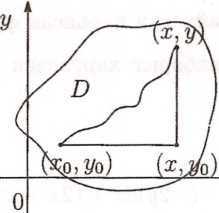
\includegraphics[width=4cm]{Zurag/5.jpg}
    \captionof{figure}{}
        \label{ref hiih ner}
\end{center}
(E-D) нөхцөл ашиглавал
\begin{eqnarray} \label{3.12}
 v(x,y)=\int\limits_{(x_0,y_0)}^{(x,y)} -\frac{\partial u}{\partial y}dx+\frac{\partial u}{\partial x}dy+C.
\end{eqnarray}
(\ref{3.12})дэх интеграл замаас хамаарахгүй, учир нь $u(x,y)$ функцийн гармоник чанар ёсоор 
$$\frac{\partial}{\partial y}\left(-\frac{\partial u}{\partial y}\right) =\frac{\partial}{\partial x}\left(\frac{\partial u}{\partial x}\right)$$
нөхцөл биелэгдэнэ. 

Гармоник $v=v(x,y)$ функц $D$-д өгөгдсөн байвал түүнтэй хосмог гармоник $u(x,y)$ функц
\begin{eqnarray}
 u(x,y)=\int\limits_{(x_0,y_0)}^{(x,y)} \frac{\partial v}{\partial y}dx-\frac{\partial v}{\partial x}dy+C
\end{eqnarray}
гэж олдох нь мэдээж.
\begin{exm}
 $u=x^2-y^2+2x$ функцээр голоморф $f(z)=u+iv$ функцийг $f(i)=2i-1$ нөхцөлд байгуул.
\end{exm}
\begin{sol}
$$\frac{\partial u}{\partial x}=2x+2,\quad \frac{\partial^2 u}{\partial x^2}=2, \quad \frac{\partial u}{\partial y}=-2y, \quad \frac{\partial^2 y}{\partial y^2}=-2$$ болж $\forall x$, $\forall y$ ийн хувьд $\Delta u=0$ байх тул дурдсан функц нийт $Oxy$ дээр гармоник байх ба хялбарыг харгалзан $x_0=0$, $y_0=0$ гэе.
(\ref{3.12}) ёсоор
\begin{eqnarray} \label{3.14}
 v(x,y)=\int\limits_{(0,0)}^{(x,y)} -(-2y)dx+(2x+2)dy+C
\end{eqnarray} болно. $\dfrac{\partial }{\partial x}\left(\dfrac{\partial u}{\partial x}\right) =\dfrac{\partial }{\partial y}\left( -\dfrac{\partial u}{\partial y}\right)$ 
байх тул (\ref{3.14}) нь замаас хамаарахгүй, зураг 6-д үзүүлснээр $OA\cup AB$ замаар интегралчилж $v(x,y)$ функцийг бодож гаргана. \\

    \begin{figure}[h]
    \centering
\begin{tikzpicture}[line cap=round,line join=round,>=triangle 45,x=1cm,y=1cm]
\clip(0,0) rectangle (6,4.5);
\coordinate (x1) at (0,1);
\coordinate (y1) at (1,0);
\coordinate (x2) at (5.5,1);
\coordinate (y2) at (1,4);
\coordinate (o) at (1,1);
\coordinate (z) at (4,3);
\draw[-stealth,line width=1pt] (x1)  -- (x2) node[right] {$x$};
\draw[-stealth,line width=1pt] (y1)  -- (y2) node[right] {$y$};
\draw (o) node[anchor=north east] {$O$};
\draw[-stealth,line width=1pt] (4,1) node[below] {$A$} -- (z) node[above right ] {$B(x,y)$};
\draw[-stealth,line width=1pt] (o)  -- (4,1);
\end{tikzpicture}
    \captionof{figure}{}
        \label{ref hiih ner}
\end{figure}
Иймд 
$$z\in OA: 0\leq x, \quad y=0 \Rightarrow dy=0,$$
$$z\in AB: x=const \Rightarrow dx=0, \quad 0\leq y$$ болж 
$$v(x,y)=\int\limits_0^x 0\cdot dx+\int\limits_0^y (2x+2)dy+C=(2x+2)y+C$$
бөгөөд 
\begin{align*}
    f(z)&=x^2-y^2+2x+[(2x+2)y+C]i\\
    &=x^2-y^2+2xyi+2(x+iy)+Ci \\
    &= z^2+2z+Ci ,\quad f(i)=2i-1
\end{align*}
нөхцөлийг ашиглавал 
$C=0$ тул $f(z)=z^2+2z\in H(\mathbb{C}).$
\end{sol}
Голоморф функц байгуулахад муруй шугаман интеграл бодоход хүргэхгүй байж болно. Үүнийг саяын жишээн дээр харуулъя:
$$\frac{\partial v}{\partial x}=-\frac{\partial u}{\partial y}=2y\Rightarrow v(x,y)=\int 2ydx+\varphi (y)=2yx+\varphi (y)$$
тул $\dfrac{\partial v}{\partial y}=2x+\varphi ' (y)$ ба $\dfrac{\partial v}{\partial y}=\dfrac{\partial u}{\partial x}$ ёсоор 
$$2x+\varphi ' (y)=2x+2\Rightarrow \varphi ' (y)=2\Rightarrow \varphi (y)=2y+C$$
болж улмаар $v(x,y)=2xy+2y+C$ гарлаа. Цаашид нөхцөлөө ашиглан $f(z)=z^2+2z$ функцээ гаргана.
\section{Уламжлалын геометр утга. Конформ буулгалт }
Комплекс $\circled{z}$ хавтгай дээр $\Gamma$-муруй $t$ параметрт
\begin{eqnarray}
  \Gamma:z=z(t)=x(t)+iy(t), \qquad \alpha\leq t\leq \beta
\end{eqnarray}
тэгшитгэлээр, өөрөөр хэлбэл бодит аргументийн $x=x(t)$, $y=y(t)$ гэсэн параметрт тэгшитгэлээр тодорхойлогдоно.
\begin{eqnarray} \label{3.16}
  z'(t_0)=\lim\limits_{\Delta t\rightarrow 0}\frac{\Delta z(z_0)}{\Delta t}=x'(t_0)+iy'(t_0), \qquad t_0\in (\alpha, \beta)
\end{eqnarray}
бөгөөд (\ref{3.16})-аас харахад хэрэв $\exists z'(t_0)$, $z'(t_0)\neq 0$ байвал комплекс (\ref{3.16}) вектор нь $\Gamma$ муруйн $z_0=z(t_0)=(x(t_0), y(t_0))$ цэг дээр татсан шүргэгчийн дагуу чиглэнэ.

$w=f(z)$ нь $z_0$ цэг дээр голоморф функц байг. Бас \\ $w_0=f(z_0)$, $f'(z_0)\neq 0$ байг. Энэ үед $z_0$-ийн орчны $\forall z$ цэг бүр
$w_0$-ийн орчны ямар нэг $w$ цэгт бууна.

$z_0$ цэгийг дайруулан түүн дээр огтлолцсон толигор \\ $\Gamma_1:z_1=z_1(t)$, $\Gamma_2:z_2=z_2(t)$ шугам авъя. 
\begin{center}
    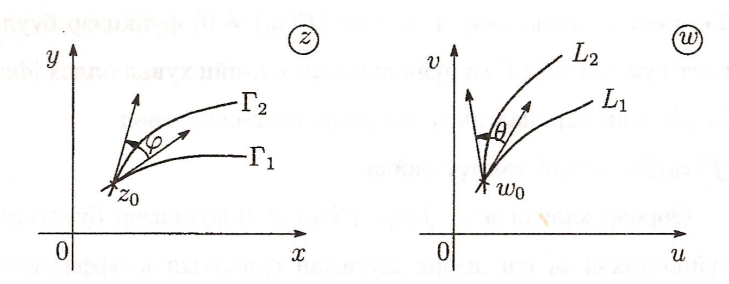
\includegraphics[width=9cm]{Zurag/7.PNG}
    \captionof{figure}{}
        \label{ref hiih ner}
\end{center}
$z_0=z_1(t_{01})$ ба $z_0=z_2t(_{02})$ байг. $w=f(z)$ буулгалтаар эдгээр шугам $\circled{w}$ дээр $w_0$ цэгт огтолцсон $L_1$, $L_2$ шугамд бууна (Зураг 7). $$L_1:w=w_1(t_1)=f(z_1(t_1));$$ $$L_2:w=w_2(t_2)=f(z_2(t_2))$$ бөгөөд харин $w_0=w_1(t_{01})=f(z_0)$; $w_0=w_2(t_{02})=f(z_0).$

Давхар $w=f[z(t)]$ функцийн уламжлалын дүрмээр:
\begin{equation} \label{3.17}
  \begin{split}
      &w'_1(t_{01})=f'(z_0)\cdot z_1'(t_{01}); \quad w'_2(t_{02})=f'(z_0)\cdot z_2'(t_{02})\\
      &dw'_1(t_{01})=f'(z_0)\cdot z_1'(t_{01})dt=f'(z_{0})\cdot dz_1(t_{01})\\
      & dw'_2(t_{02})=f'(z_0)\cdot z_2'(t_{02})dt_1=f'(z_0)\cdot dz_2(t_{02})
  \end{split}
\end{equation}
Бид одоо, уламжлалын модуль ба аргументийн геометр утгын талаар дараах хоёр теорем батлах боломжтой боллоо. 
\begin{thm}
Голоморф $w=f(z) \quad (f'(z_0)\neq 0)$ функцээр буулгалт гүйцэтгэхэд $\Gamma$ муруйн дүр болох $L$-ийн хувьд олдох $|dw|$ ба $|dz|$-ийн харьцаа нь $z_0$ цэг дээр тогтмол бөгөөд $|f'(z_0)|(>0)$-тай тэнцүү байна.

Өөрөөр хэлбэл $w=f(z)$, $f'(z_0)\neq 0$ функцээр буулгалт гүйцэтгэхэд $z_0$ цэг дээрх шугаман суналтын коэффициент нь $|f'(z_0)|$ байна.
\end{thm}
\begin{prf}
(\ref{3.17}) томьёог ашиглавал 
$$\frac{|dw_1(t_{01})|}{|dz_1(t_{01})|}=|f'(z_0)|; \qquad \frac{|dw_2(t_{02})|}{|dz_2(t_{02})|}=|f'(z_0)|$$
$\Gamma_1$ ба $\Gamma_2$ шугамыг дураараа сонгоно. 
\hfill $\blacksquare$\end{prf}
\begin{thm}
Голоморф $w=f(z)$, $f(z_0)\ne 0$ функцээр буулгалт гүйцэтгэхэд $z_0$ цэг дээрх шүргэгч векторын эргэлтийн өнцөг $\Arg  f'(z_0)$-тэй тэнцүү бөгөөд муруйнуудын $z_0$ дээрх өнцгүүд хадгалагдана.
\end{thm}
\begin{prf}
 $z_0$ цэг дээр $\Gamma_1$ ба $\Gamma_2$ шугамуудын хоорондох өнцөг (нар буруу тойролтоор тоологдох)
 $$\varphi =\Arg  dz_2(t_{02})-\Arg  dz_1(t_{01})$$
 байх бөгөөд (\ref{3.17}) ёсоор харгалзах $L_1$ ба $L_2$ муруйнуудын $w_0$ цэг дээрх $\theta$ өнцөг
\begin{align*}
    \theta&= \Arg  dw_2(t_{02})-\Arg  dw_1(t_{01}) \\
    &=\Arg  f'(z_0)+\Arg  dz_2(t_{02})-\Arg  f'(z_0)-\Arg  dz_1(t_{01})\\
    &=\Arg  dz_2(t_{02})-\Arg  dz_1(t_{01})=\varphi
\end{align*}
болж, вектор бүхний хувьд
$$\Arg  dw (t_0)=\Arg  f'(z_0)+\Arg  z(t_0)$$
байна. Теорем батлагдав. 
\hfill $\blacksquare$\end{prf}
\begin{hnt}
Энэ тохиолдолд муруйнуудын хоорондох өнцгүүд тэнцүү төдийгүй тэдгээрийн тоологдох чиглэл адилхан байна (цөм нар буруу тойрч тоологдох).
\end{hnt}
\begin{dfn}
$z_0$ цэгийг дайрсан муруйнуудын хоорондох өнцгийг хэвээр хадгалж, чиглэл бүрдээ шугаман суналт тогтмол байх $w=f(z)$ буулгалтыг $z_0$ цэг дээр конформ буулгалт \index{Конформ буулгалт} гэнэ. Өнцгийн тоологдох чиглэл таарч байвал I төрлийн, \index{I төрлийн конформ буулгалт} эсрэг байвал II төрлийн конформ буулгалт \index{II төрлийн конформ буулгалт} гэдэг. 
\end{dfn}
\begin{thm}
$w=f(z)$ функц $z_0$ цэг дээр голоморф бөгөөд $f'(z_0)\neq 0$ байвал тэр нь $z_0$ цэг дээр конформ буулгалт өгнө.

$D$ мужийн цэг бүр дээр конформ $w=f(z)$ буулгалтыг $D$ дээр конформ гэнэ. $D$ муж дээр голоморф $w=f(z)$ функц $D$ мужийг $D^*$ муж руу конформ буулгахын тулд $\forall z\in D$ дээр $f'(z)\neq 0$, түүнчлэн $D$ дээр уул функц нэг хуудаст $(\forall z_1,z_2\in D$ үед $f(z_1)\neq f(z_2)$ байх нь зөвхөн $z_1\neq z_2$ үед) байхыг шаардана.
\end{thm}
\begin{hnt}
$w=f(z)$ функц $z_0$ цэгийн ямар нэг орчинд нэг хуудаст байвал $z_0$ цэг дээр нэг хуудаст гэнэ. Голоморф $w=f(z)$ функц $f'(z_0)\neq 0$ байвал тэр нь $z_0$ дээр нэг хуудаст байна. Харин $D$ мужид нэлэнхийдээ $f'(z)\neq 0$ байхаас $w=f(z)$ функц $D$ дээр нэг хуудаст байх нь алба биш. Жишээ нь $w=z^2$ функц цагираг хэлбэрийн $D:1<|z|<2$ мужийн цэг бүр дээр нэг хуудаст боловч тэр нь $D$-дээр нэг хуудаст биш. Учир нь $\forall z\in D$-ийн хувьд $f(-z)=f(z)$ байна. 
\end{hnt}
\begin{exm}
$f(z)=z^2$ буулгалтын $1+\sqrt{3}i$ цэг дээрх шугаман суналтын коэффициент ба эргэлтийн өнцгийг ол.
\end{exm}
\begin{sol}
$w'=2z$, $|2(1+\sqrt{3}i)|=4$, $\arg  2(1+\sqrt{3}i)=\dfrac{\pi}{3}.$\\ $f(z)=z^2$ функц нийт $\mathbb{C}$ дээр голоморф бөгөөд $z_0$ дээр конформ буулгалт өгнө.
$$|f'(1+\sqrt{3}i)|=4, \quad \arg  f'(1+\sqrt{3}i)=\frac{\pi}{3}$$ тул өгөгдсөн цэг дээр шугаман суналтын коэффициент 4 ба $\dfrac{\pi}{3}$ өнцгөөр эргэлт явагдана.
\end{sol}
\begin{exm}
$w=\sin z$ функц $1+i$ цэг дээр ямар суналт, эргэлт өгөх вэ?
\end{exm}
\begin{sol}
$w'=\cos z$ тул $k=|\cos (1+i)|=\sqrt{ \ch^2 1-\sin^2 1}$; \qquad $\theta = \arccos (1+i)=-\arctan 11$ байна. 
\end{sol}
\begin{center}
    Дасгал
\end{center}
\begin{enumerate}
    \item [13.]
    Дараах функцийн бодит ба хуурмаг хэсгийг ол.
    \colgur
    {\begin{enumerate}
        \item [a)] $w=z^3,$
        \item [b)] $w=ze^{-z},$
        \item [c)] $w=\sin\overline{z}.$
    
    \end{enumerate}}
    \item[14.] Дараах функцийн бодит ба хуурмаг хэсгийг ол.
    \colgur{
    \begin{enumerate}
    \item [a)]$\sin z$
    \item [b)] $ch z$
    \item[c)] $\Ln i$
    \item [d)] $ln (1-i)$
    \item [e)] $2^i$
    \item [(f)] $(1+i)^i$
    \end{enumerate}
    }
    \item[15.] Мэдэгдэж байгаа бодит буюу хуурмаг хэсгээр голоморф функц $w= f(z)$ байгуул.
    \begin{enumerate}[a)]
        \item  $u=\dfrac{x}{x^2+y^2}, \qquad f(\pi)=\dfrac{1}{\pi}$
        \item $v=xy-2y, \qquad f(0)=0$
        \item $v=2 \ch x \sh y-xy, \qquad f(0)=0.$
    \end{enumerate}
\end{enumerate}